\documentclass{article}
\usepackage{graphicx} % Required for inserting images
\usepackage{verbatim}
\usepackage{amsmath}
\usepackage{algorithmicx}
\usepackage{algpseudocode}
\usepackage{array}
\usepackage{booktabs}


\usepackage{algorithm}



\title{DMA problemset 2}
\author{Daniel Andre Bunckenburg - tvf882@alumni.ku.dk}
\date{February 2025}

\begin{document}

\maketitle

\newpage

\section{Opgave 1}

\begin{figure}[htbp]
    \centering
    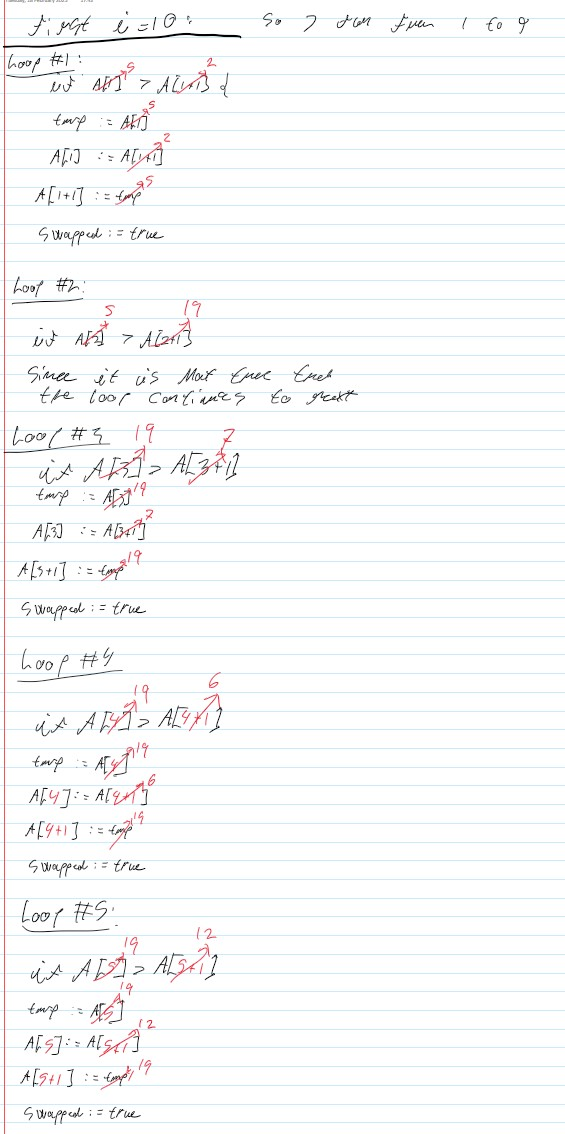
\includegraphics[width=0.8\textwidth]{Figures/problemset2_1.jpg}
    \caption{Caption for the figure.}
    \label{fig:myfigure}
\end{figure}

\begin{figure}[h!]
    \centering
    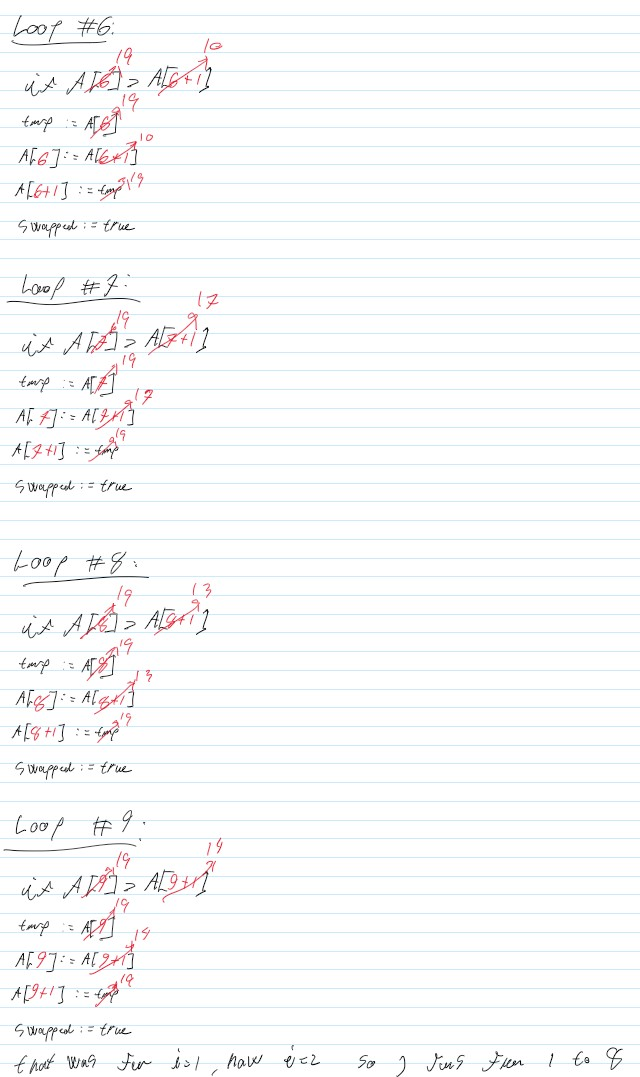
\includegraphics[width=0.8\textwidth]{Figures/problemset2_2.jpg}
    \caption{Caption for the figure.}
    \label{fig:myfigure}
\end{figure}



\begin{verbatim}

j := n
good := True
while (j > 1 and good) 
    i := j - 1
    while (i >= 1 and good)
        if (A[i] > A[j])
            good := false
        i := i - 1
    j := j - 1
if (good)
    return "Success"
else
    return "failure"

\end{verbatim}



\newpage
\section{Part 2}


\subsection{a}

The thing that went wrong was that the number of kids was odd and not even. 


If looking at my drawing you see two senarios, the first is if there is an even amount of kids. Then it is possible to position the kids in a way that they are each orther closes, then it is called a mutual 2-cycles and it is possible to that all kids recives a ball, like 
\[
A \to B \quad \text{and} \quad B \to A.
\]

in the orther case there allways be one kid left without any ball.


\begin{figure}[h!]
    \centering
    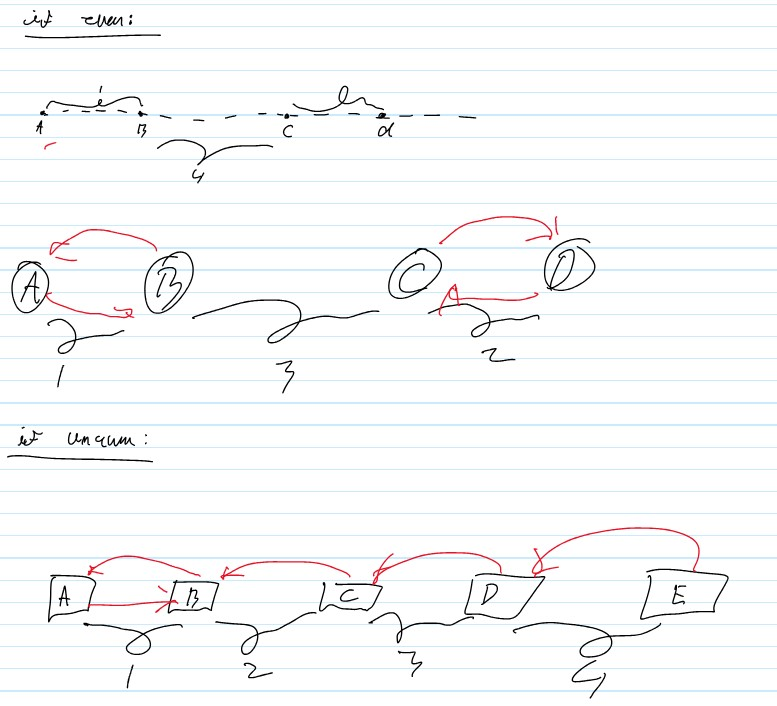
\includegraphics[width=0.8\textwidth]{Figures/figure_1.jpg}
    \caption{Caption for the figure.}
    \label{fig:myfigure}
\end{figure}





What went wrong? Was Jakob just immensely unlucky? Or can you prove mathematically
that it was unavoidable that at least one child would end up without a ball? Would this
had been different if Jakob had not insisted on 51 children, but had accepted the proposal
by his colleagues to have 50 children? Or if not all distances would have had to be different?

\end{document}
